\documentclass{article}
\usepackage{a4wide}


\usepackage{polski}
\usepackage[utf8x]{inputenc}
\usepackage{graphicx}
\usepackage{float}
\usepackage{hyperref}
\usepackage{listings}
\usepackage{mathtools}
\usepackage{amsmath}

\usepackage{color} %red, green, blue, yellow, cyan, magenta, black, white
\definecolor{mygreen}{RGB}{28,172,0} % color values Red, Green, Blue
\definecolor{taupe}{rgb}{0.28, 0.24, 0.2}
\definecolor{mylilas}{RGB}{0,110,0}


\author{Lev Sergeyev}
\title{SPC. Ćwiczenie 5. Estymacja. Metoda NK}

\date{06.12.2019, pt/TN 13:15}
\begin{document}

\maketitle

%\pagebreak


\section{Standardowa metoda NK (wersja off-line)}
\par
Dany jest obiekt:
\begin{equation}
y_n=a_1^* y_{n-1} + a_2^* y_{n-2} + b_0^* u_n + b_1^* u_{n-1} + z_n
\end{equation}
Gdzie \( \mathbf{E}z = 0  \) \\
Dla obiektu dobrano takie parametry A i B, aby obiekt był stabilny:

\begin{equation}
\Theta^* = \begin{bmatrix}
a_1^* \\ a_2^* \\ b_0^* \\ b_1^*
\end{bmatrix} = \begin{bmatrix}
0.4 \\ 0.3 \\ 1 \\ 1
\end{bmatrix}
\end{equation}

Następnie, używając metody najmniejszych kwadratów, przeprowadzono estymację parametrów w obecności zakłóceń:

\begin{equation}
\Phi_N = \begin{bmatrix}
Y_{N-1} & Y_{N-2} & U_N & U_{N-1}
\end{bmatrix}
 = \begin{bmatrix}
y_{0} & y_{-1} & u_1 & U_{0} \\ 
y_{1} & y_{0} & u_2 & U_{1} \\ 
\vdots & \vdots & \vdots & \vdots \\ 
y_{n-1} & y_{n-2} & u_n & U_{n-1} 
\end{bmatrix}
\end{equation}

\begin{equation}
\widehat{\Theta} = (\Phi_N^T \Phi_N)^{-1} \Phi_N^T Y_N = \begin{bmatrix}
0.398 \\  0.3 \\ 0.985 \\ 1.02
\end{bmatrix}
\end{equation}

%\pagebreak

\section{Rekurencyjna metoda NK (wersja on-line)}

\begin{equation}
\widehat{\Theta}_n = \widehat{\Theta}_{n-1} + P_n \phi_n ( y_n - \phi_n^T \widehat{\Theta}_{n-1} )
\end{equation}

\begin{equation}
P_n = P_{n-1} - \frac{P_{n-1} \phi_n \phi_n^T  P_{n-1}}{1 + \phi_n^T P_{n-1} \phi_n}
\end{equation}

\begin{equation}
\phi_n = \begin{bmatrix}
y_{n-1} \\ y_{n-2} \\ u_n \\ u_{n-1}
\end{bmatrix}
,
\widehat{\Theta}_0 =  \begin{bmatrix}
0 \\  0 \\ 0 \\ 0
\end{bmatrix}
,
P_0= \begin{bmatrix}
1000 & 0 & 0 & 0 \\ 
0 & 1000 & 0 & 0 \\ 
0 & 0 & 1000 & 0 \\ 
0 & 0 & 0 & 1000 
\end{bmatrix}
\end{equation}

\pagebreak

\begin{figure}[ht]
\centering
\scalebox{0.35}{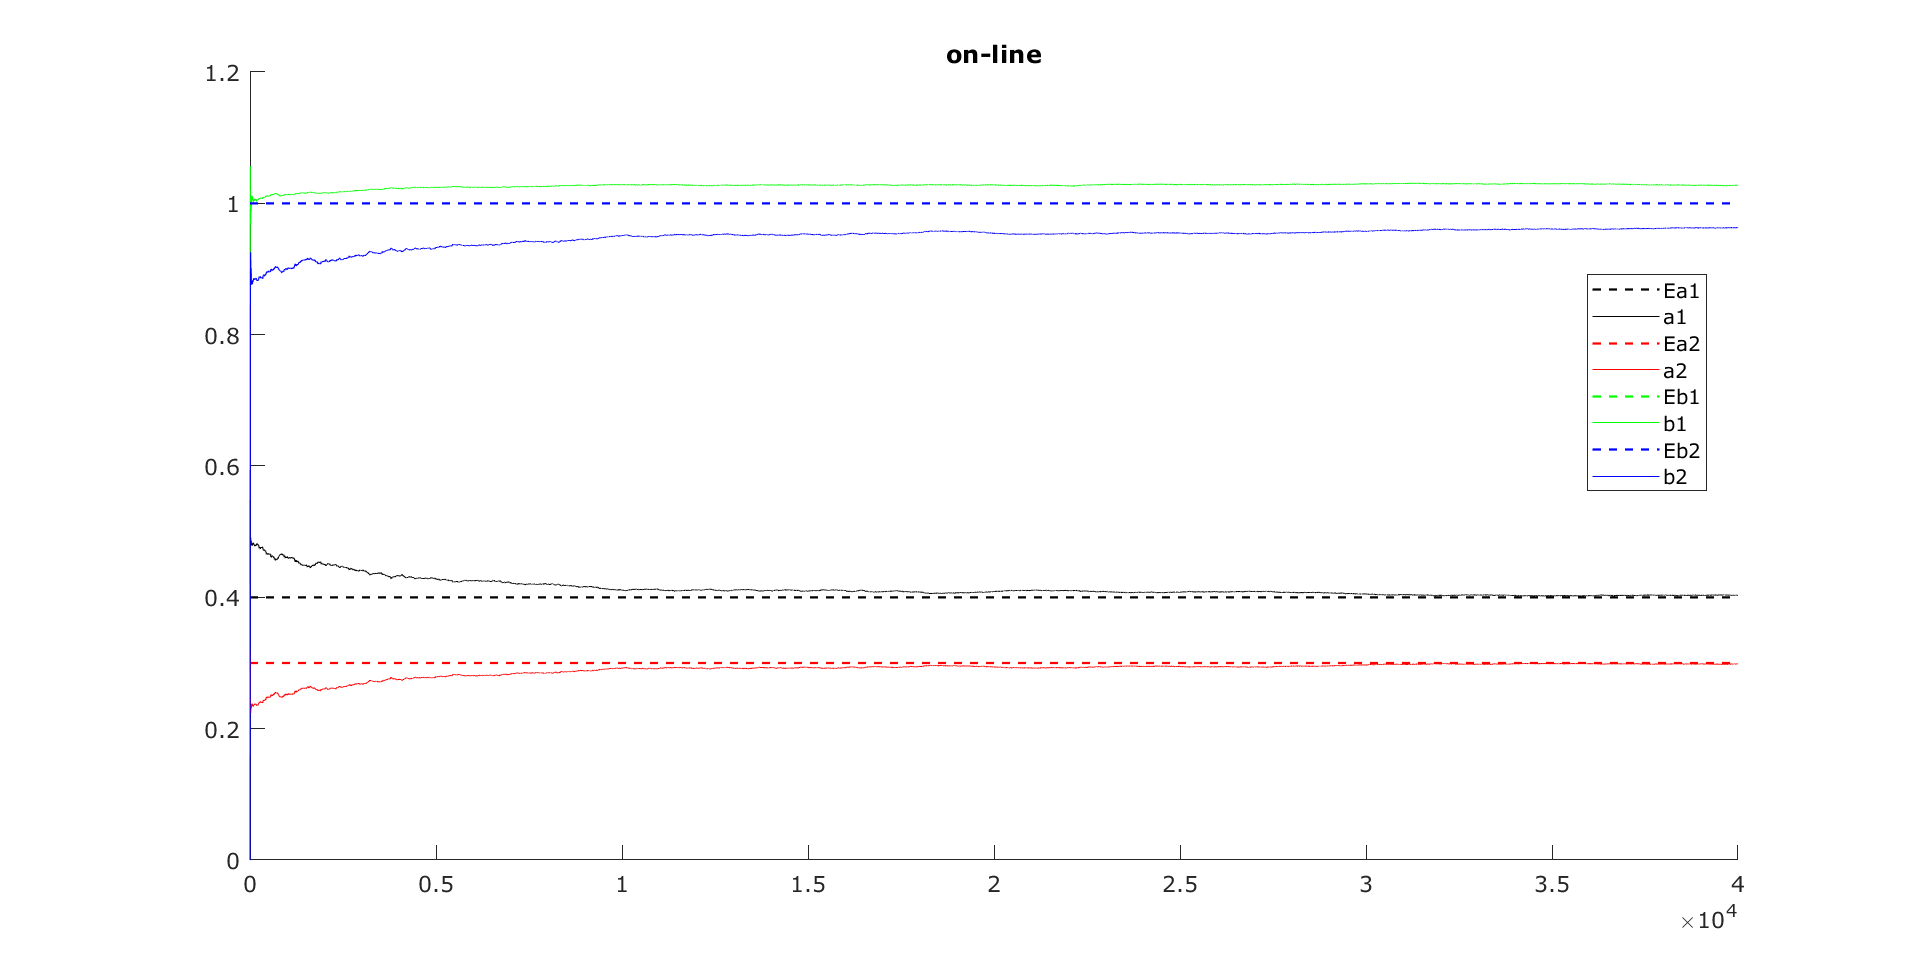
\includegraphics{online.png}}
\caption{Estymacja metodą NK on-line}
\end{figure}


\subsection{Ważona metoda NK}
Do rekurencyjnej metody najmniejszych kwadratów dodana została waga \( \lambda \):

\begin{equation}
P_n = \frac{1}{\lambda} (P_{n-1} - \frac{P_{n-1} \phi_n \phi_n^T  P_{n-1}}{\lambda + \phi_n^T P_{n-1} \phi_n} )
\end{equation}

\subsection{Obiekt stacjonarny}

Dla \( \lambda = 0.9999 \):

\begin{figure}[ht]
\centering
\scalebox{0.35}{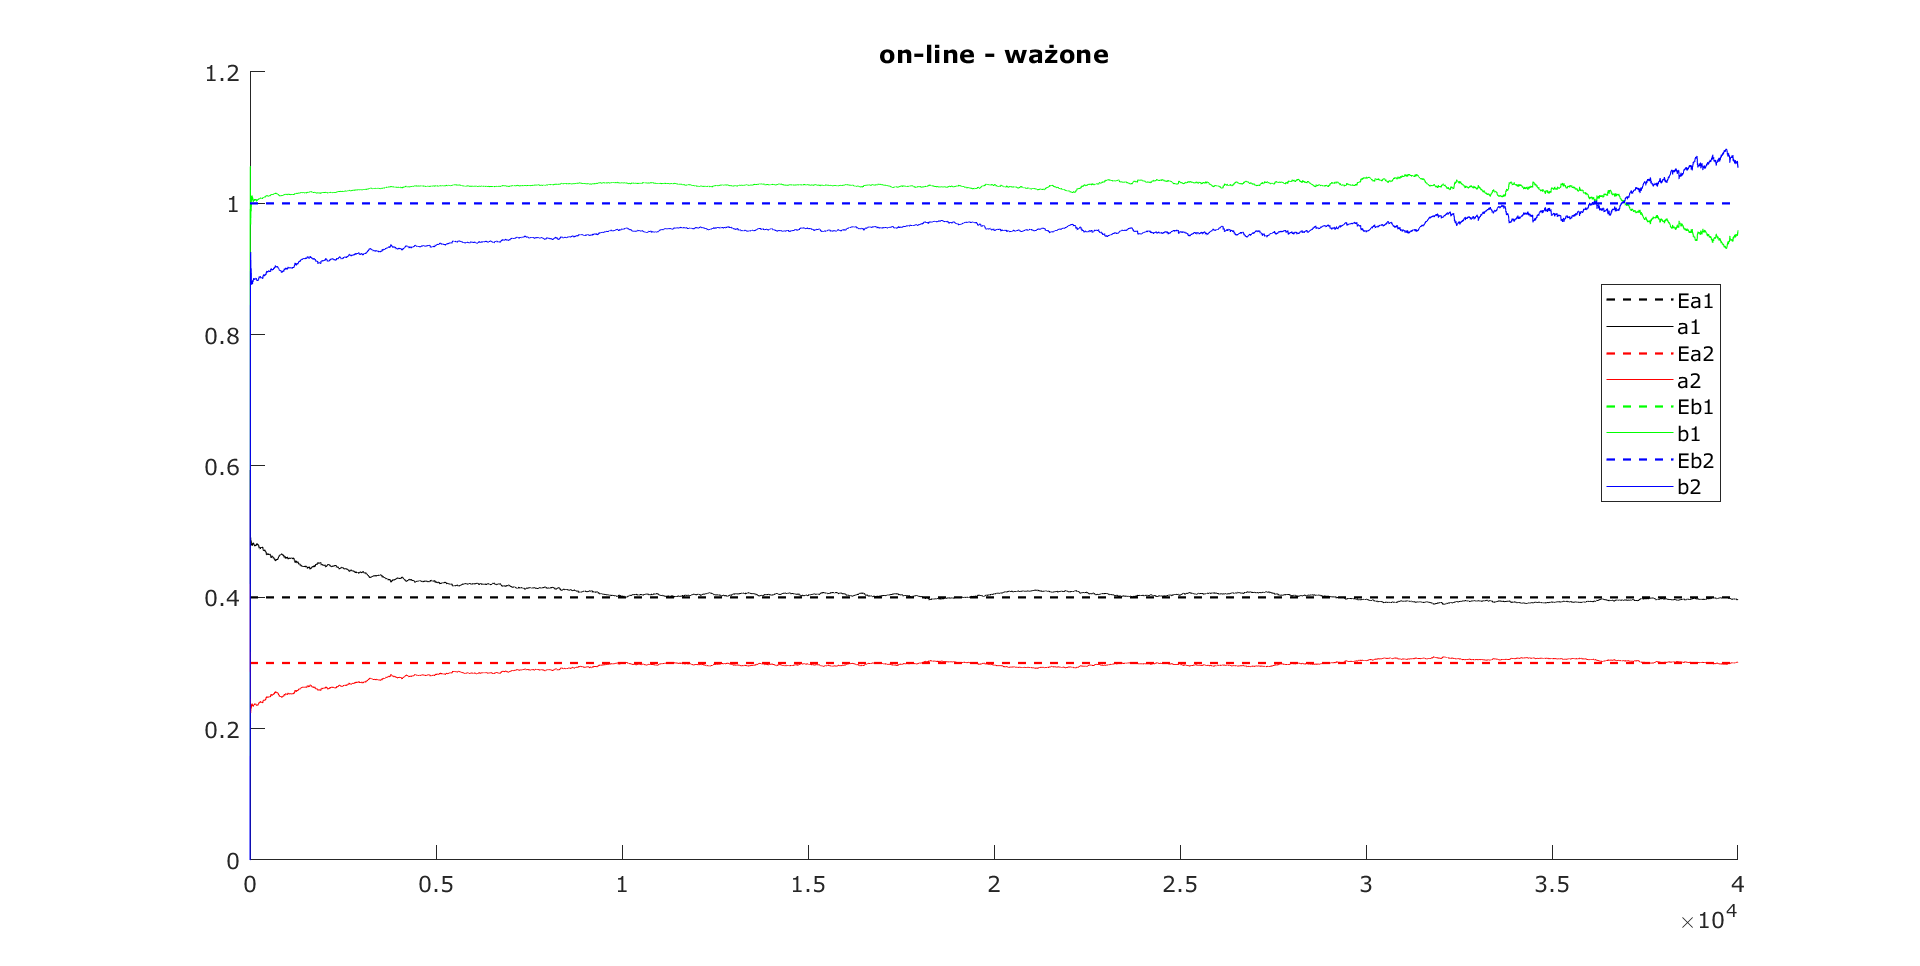
\includegraphics{onlineW.png}}
\caption{Estymacja metodą ważoną NK on-line}
\end{figure}

\subsection{Obiekt niestacjonarny}

Dla \( \lambda = 0.9999 \):

\begin{figure}[ht]
\centering
\scalebox{0.35}{\includegraphics{onlineWNS.png}}
\caption{Estymacja metodą ważoną NK on-line}
\end{figure}

Dla \( \lambda = 0.999 \):

\begin{figure}[ht]
\centering
\scalebox{0.35}{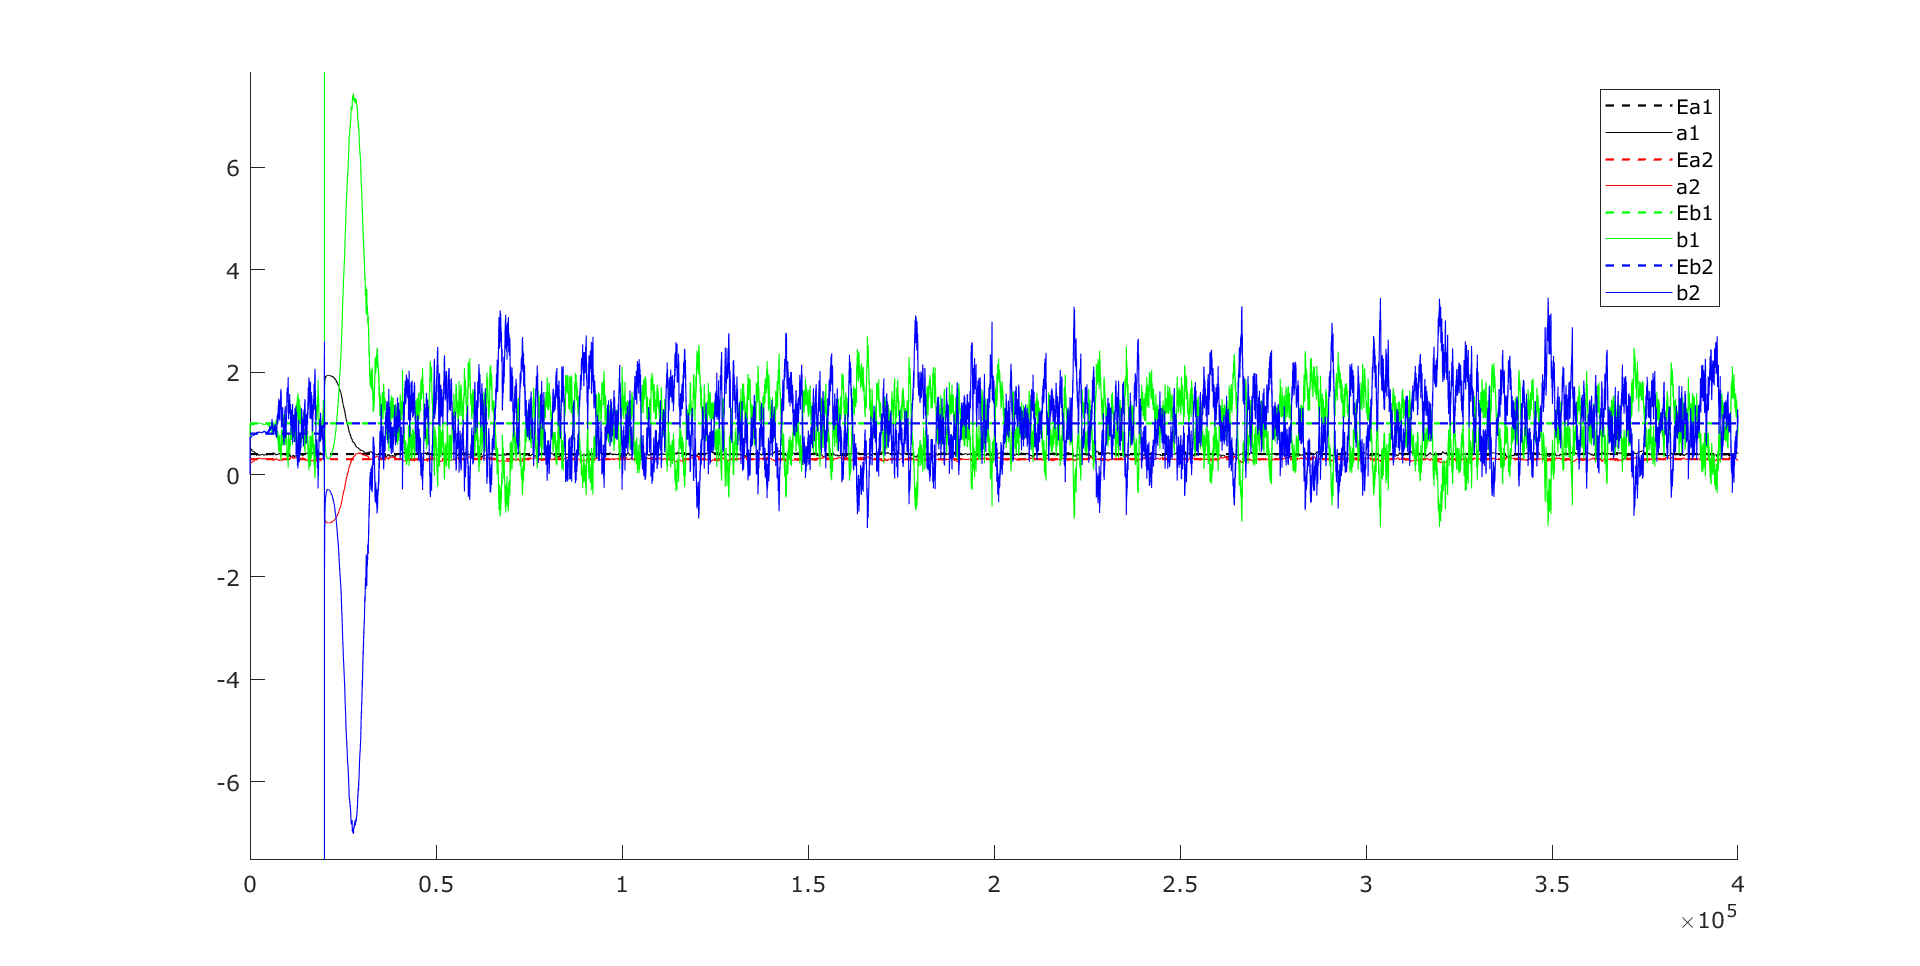
\includegraphics{onlineWNSl.png}}
\caption{Estymacja metodą ważoną NK on-line}
\end{figure}
\section{Wnioski}

Wynik uzyskany po estymacji motodą NK off-line wskazuje na skuteczność użytej metody.
\par
Dla rekurencyjnej metody NK wynik na końcu jest zbliżony do metody standardowej, ale zależy od warunków początkowych w tym od \( \widehat{\Theta}_0 \), źle dobrane warunki początkowe mogą sprowadzić do wydłużenia czasu uzyskania poprawnego wyniku. Taka metoda nadaje się tylko do obiektów stacjonarnych, gdyź kumuluje wszystkie dotychczasowe pomiary z równą wagą.
\par
Wprowadzenie wagi dla starszych pomiarów rozwiązuje powyżej opisany problem. Dla mniejszej \( \lambda \) jest szybsza adaptacja, ale estymator jest bardziej poddatny na zakłócenia. 

\end{document}


